\documentclass{beamer}
\usepackage{beamerthemesplit}
\usepackage{wrapfig}
\usetheme{SPbGU}
\usepackage{pdfpages}
\usepackage{amsmath}
\usepackage{cmap} 
\usepackage[T2A]{fontenc} 
\usepackage[utf8]{inputenc}
\usepackage[english,russian]{babel}
\usepackage{indentfirst}
\usepackage{amsmath}
\usepackage{tikz}
\usepackage{multirow}
\usepackage[noend]{algpseudocode}
\usepackage{algorithm}
\usepackage{algorithmicx}
\usetikzlibrary{shapes,arrows}
\usepackage{fancyvrb}
\newtheorem{rutheorem}{Теорема}
\newtheorem{ruproof}{Доказательство}
\newtheorem{rudefinition}{Определение}
\newtheorem{rulemma}{Лемма}
\beamertemplatenavigationsymbolsempty

\title[]{Теория автоматов и формальных языков}
\subtitle[]{Введение}
\institute[]{
Санкт-Петербургский государственный электротехнический университет <<ЛЭТИ>>\\
}

\author[]{Екатерина Вербицкая}

\date{ сентября 2016г.}

\definecolor{orange}{RGB}{179,36,31}

\begin{document}
{
  \begin{frame}
    \titlepage
  \end{frame}
}


\begin{frame}[fragile]
  \transwipe[direction=90]
  \frametitle{Контекст: языки}
  \begin{itemize}
    \item Естественные 
    \begin{itemize}
      \item Русский, английский...
    \end{itemize}    
    \pause
    \item Искусственные
    \begin{itemize}
      \item Эсперанто, ложбан...
      \item Клингонский, эльфийский...
      \pause
      \item C++, Java, C\#, Haskell, OCaml, Perl, Coq, Agda...
    \end{itemize}
  \end{itemize}
\end{frame}
            

\begin{frame}[fragile]
  \transwipe[direction=90]
  \frametitle{Контекст: языковые процессоры}
  \begin{itemize}
    \item Текстовые редакторы
    \item Компиляторы, интерпретаторы, трансляторы
    \item Среды разработки
  \end{itemize}

  \begin{itemize}
    \item Все нуждаются в некотором формализованном представлении языка
  \end{itemize}
\end{frame}

\begin{frame}[fragile]
  \transwipe[direction=90]
  \frametitle{Язык программирования}
  \begin{itemize}
    \item Синтаксис --- правила построения программ из символов
    \item Семантика --- правила истолкования программ, определяющие их смысл
  \end{itemize}
\end{frame}


\begin{frame}[fragile]
  \transwipe[direction=90]
  \frametitle{Пример: язык арифметических выражений}
  \begin{itemize}
    \item Алфавит символов: цифры, скобки, знаки арифметических операций $(+, -, *, /)$
    \item Синтаксис
    \begin{itemize}
      \item \textbf{Терм}: последовательность цифр или любое \textbf{выражение} в скобках
      \item \textbf{Слагаемое}: последовательность \textbf{термов}, соединненых знаками умножения и деления
      \item \textbf{Выражение}: последовательность \textbf{слагаемых}, соединенных знаками сложения и вычитания (перед первым \textbf{слагаемым} может стоять минус)
    \end{itemize}
    \item Семантика
    \begin{itemize}
      \item Значение выражения
    \end{itemize}
  \end{itemize}
\end{frame}

\begin{frame}[fragile]
  \transwipe[direction=90]
  \frametitle{Метаязык}
  \begin{itemize}
    \item Язык, на котором дано описание языка
    \begin{itemize}
      \item Естественный язык
      \pause
      \item Язык металингвистичесих формул Бэкуса (БНФ)
      \pause \item Синтаксические диаграммы
      \pause \item Грамматики...
    \end{itemize}
  \end{itemize}
\end{frame}

\begin{frame}[fragile]
  \transwipe[direction=90]
  \frametitle{Алфавит}
  \begin{itemize}
    \item \textbf{Алфавит} --- конечное множество символов
    \begin{itemize}
      \item $\{ a, b, c, \dots, z \}$
      \item $\{ \alpha, \beta, \gamma, \dots, \omega \}$
      \item $\{ 0, 1 \}$
      \item $\{$ \underline{let}, \underline{in}, \underline{where}, \dots $\}$
    \end{itemize}    
  \end{itemize}
\end{frame}

\begin{frame}[fragile]
  \transwipe[direction=90]
  \frametitle{Цепочка}
  \begin{itemize}
    \item \textbf{Цепочка (предложение, слово)} --- любая конечная 
последовательность символов алфавита
    \begin{itemize}
      \item cat
      \item $\kappa \alpha \tau$
      \item 011000110110000101110100
      \item \verb!main = putStrLn . show . inc 2 where inc = \x -> x + 1!
    \end{itemize}    
    \item \textbf{Пустая цепочка $\varepsilon$} --- цепочка, не содержащая ни одного символа
    \begin{itemize}
      \item $\varepsilon$ не является символом алфавита
    \end{itemize}   
  \end{itemize}
\end{frame}

\begin{frame}[fragile]
  \transwipe[direction=90]
  \frametitle{Конкатенация строк}
  \begin{itemize}
    \item \textbf{Конкатенация строк $\alpha$ и $\beta$ $(\alpha \cdot \beta = \alpha \beta)$} --- результат 
приписывания строки $\beta$ в конец строки $\alpha$
    \begin{itemize}
      \item $\forall \alpha \beta \gamma. (\alpha \cdot \beta) \cdot \gamma = \alpha \cdot (\beta \cdot \gamma)$
      \item $\forall \alpha. \alpha \cdot \varepsilon = \varepsilon \cdot \alpha = \alpha$
    \end{itemize}
  \end{itemize}
\end{frame}

\begin{frame}[fragile]
  \transwipe[direction=90]
  \frametitle{БНФ ---  Бэкуса-Наура форма}
  \begin{itemize}
    \item \textbf{Символ} --- элементарное понятие языка
    \begin{itemize}
      \item $+$ означает сложение в языке арифметических выражений
    \end{itemize}
    \item \textbf{Метапеременная} --- сложное понятие языка
    \begin{itemize}
      \item Переменной <выражение> можно обозначить выражение
    \end{itemize}
    \item \textbf{Формула}
    \begin{itemize}
      \item $<$определяемый символ$> ::= <$посл$.1> | \dots | <$посл$.n>$
      \item В правой части формулы --- альтернатива конкатенаций строк, составленных из символов и метапеременных
    \end{itemize}  
    \item Пример: число
    \begin{itemize}
      \item $<$число$> ::= <$цифра$> \, | \, <$цифра$><$число$>$ 
    \end{itemize}
  \end{itemize}  
\end{frame}
    
 \begin{frame}[fragile]
   \transwipe[direction=90]
   \frametitle{Расширенная форма Бэкуса Наура (EBNF)}
   \begin{itemize}
     \item Более емкие операции
      \item \textbf{Итерация}  
      \begin{itemize}
        \item $<$x$> \, ::= \{ <$y$> \}$ эквивалентно: $<$x$> \, ::= \varepsilon \, | <$y$><$x$>$
      \end{itemize}   
      \item \textbf{Условное вхождение}  
      \begin{itemize}
        \item $<$x$> \, ::= [ <$y$> ]$ эквивалентно: $<$x$> \, ::= \varepsilon \, | <$y$>$
      \end{itemize}  
      \item Скобки для группировки
      \begin{itemize}
        \item $(<$x$> \, | \, <$y$>) <$z$>$ эквивалентно: $<$x$><$z$> \, | \, <$y$><$z$>$
      \end{itemize} 
  \end{itemize}
\end{frame}

\begin{frame}[fragile]
  \transwipe[direction=90]
  \frametitle{Пример: арифметические выражения}

$$
\begin{array}{crcl}
&<expr>& ::= & [-] <factor> \{ <+-> \, <factor> \} \\
&<+->& ::= & + \, | \, - \\
&<factor>& ::= & <term> \{ <*/> \, <term> \} \\
&<*/>& ::= & * \, | \, / \\
&<term>& ::= & <number> \, | \, ( <expr> )
\end{array}
$$

\end{frame}

\begin{frame}[fragile]
  \transwipe[direction=90]
  \frametitle{Синтаксические диаграммы Вирта}
\begin{center}
  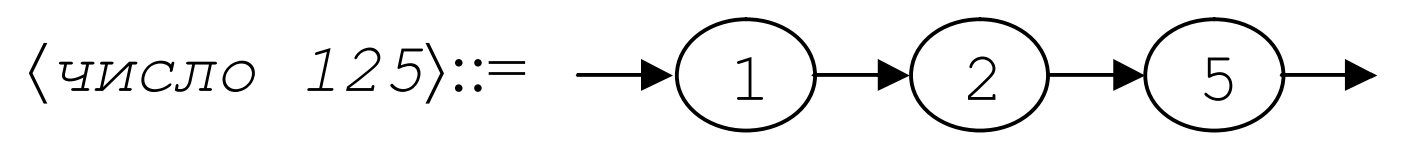
\includegraphics[width=0.65\textwidth]{pics/sdseq.png}  \\~\\     \pause
  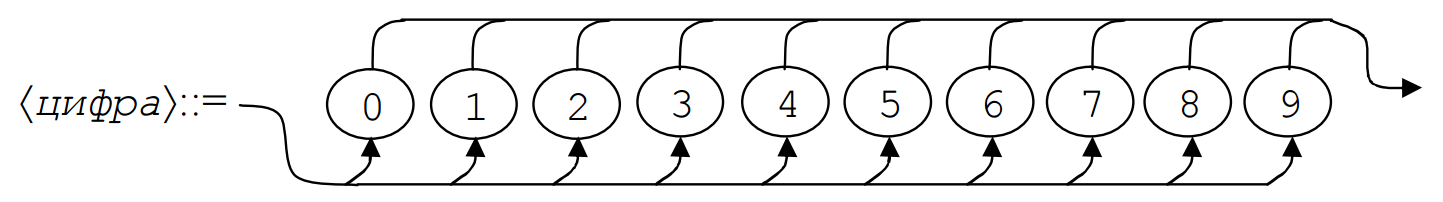
\includegraphics[width=1.0\textwidth]{pics/sddig.png}  \\~\\  \pause   
  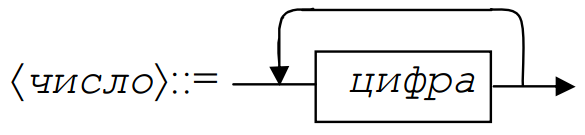
\includegraphics[width=0.45\textwidth]{pics/sdnum.png}  
\end{center}
\end{frame}


\begin{frame}[fragile]
  \transwipe[direction=90]
  \frametitle{Синтаксические диаграммы Вирта}
\begin{center}
  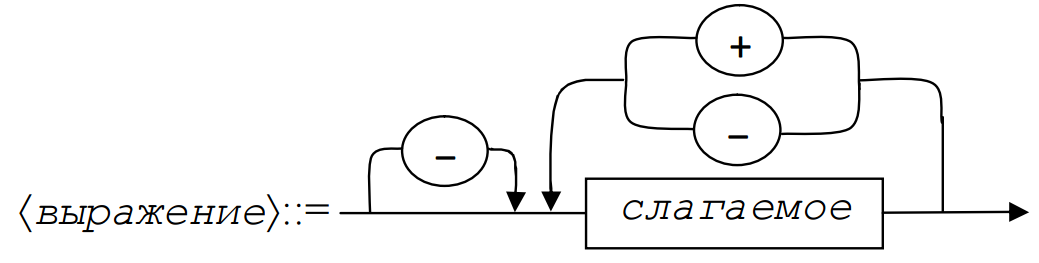
\includegraphics[width=0.75\textwidth]{pics/sdexpr.png}  \\~\\     \pause
  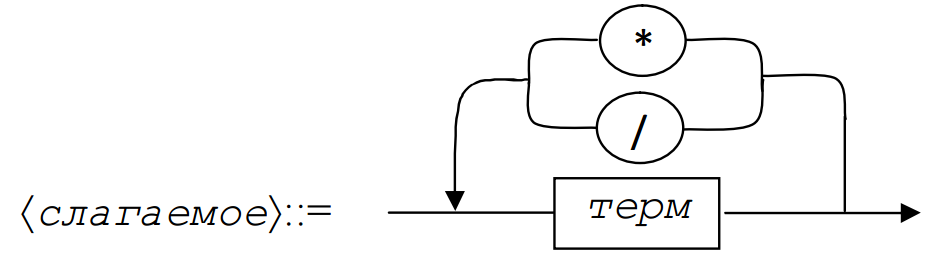
\includegraphics[width=0.75\textwidth]{pics/sdfact.png}  \\~\\  \pause   
  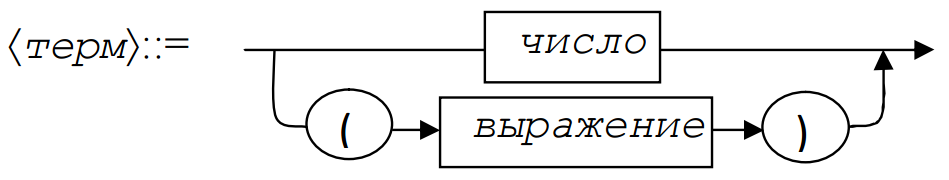
\includegraphics[width=0.75\textwidth]{pics/sdterm.png}  
\end{center}
\end{frame}

\begin{frame}[fragile]
  \transwipe[direction=90]
  \frametitle{Операции над строками}
  \begin{itemize}
    \item \textbf{Обращение (реверс) цепочки $a^R$} --- цепочка, символы которой записаны в обратном порядке
    \begin{itemize}
      \item Если $x = abc$, $x^R = cba$
      \item $\varepsilon^R = \varepsilon$
    \end{itemize}
    \item \textbf{$n-$я степень цепочки $a^n$} --- конкатенация $n$ повторений цепочки
    \begin{itemize}
      \item $a^0 = \varepsilon$
      \item $a^n = a \cdot a^{n-1} = a^{n-1} \cdot a$
    \end{itemize}
    \item \textbf{Длина цепочки $|a|$} --- количество составляющих ее символов
    \begin{itemize}
      \item $|babb| = 4, |babb|_a = 1, |babb|_b = 3, |babb|_c = 0$
      \item $|\varepsilon| = 0$
    \end{itemize}
  \end{itemize}
\end{frame}

\begin{frame}[fragile]
  \transwipe[direction=90]
  \frametitle{Формальный язык}
  \begin{itemize}
    \item $V$ --- алфавит
    \begin{itemize}
      \item $V = \{ 0, 1 \}$
    \end{itemize}
    \item $V^*$ --- множество, содержащее все цепочки в алфавите V, включая пустую цепочку
    \begin{itemize}
      \item $V^*=  \{ \varepsilon, 0, 1, 00, 11, 01, 10, 000, 001, 011, ... \}$
    \end{itemize}
    \item $V^+ = V^* \setminus \{ \varepsilon \} $ 
    \begin{itemize}
      \item $V^+ = \{0, 1, 00, 11, 01, 10, 000, 001, 011, \dots \}$
    \end{itemize}
    \item $Язык в алфавите V$ --- подмножество множества всех цепочек в этом алфавите. 
    \begin{itemize} 
      \item Для любого языка $L$ справедливо $L \in V^*$
    \end{itemize}
  \end{itemize}
\end{frame}


\begin{frame}[fragile]
  \transwipe[direction=90]
  \frametitle{}
  \begin{itemize}
    \item 
  \end{itemize}
\end{frame}


\end{document}
